\chapter{Experimental Results}

In this chapter, we present the results that we acquired while testing our method. We tested our method using real datasets collected from 1000 Genome Project and Turkish Genome Project. Since there is no validated results for paralog genes, we compare our results with the results of mrCaNaVaR \cite{alkan2009personalized}, a tool to discover structural variations in duplicated regions. mrCaNaVaR, like our method, was based on read depth and it was designed to determine absolute copy numbers in duplicated regions \cite{kahveci2018whole}. However it requires a sequence alignment file with multiple read mapping, such as mrFAST \cite{alkan2009personalized}.


\section{Datasets}
We tested our method with two human genomes: NA12878 from 1000 Genome project and 42S291210 from Turkish Genome project. In general, 30X sequencing coverage is adequate for clinical-level research \cite{shevchenko2016clinical}. Therefore we picked one genome (NA12878) as an example of a human genome sequence with a high coverage (43x) and another genome (42S291210) as an example of relatively low coverage genome (20x).

\section{Results}
In this section, the results of mrCaNaVaR and our method are compared via several plots. The results include absolute copy numbers of paralog genes (i.e. genes overlapping with segmental duplications). It is not expected the results to match perfectly, however, they should show some level of consistency. We measure the consistency as overlapping percentages. The overlapping percentages are the ratio of absolute copy numbers. For example, the \%90 or more overlapping are calculated  as; $$\frac{90}{100} \leq \frac{CNV_{our\_method}}{CNV_{mrCaNaVaR}} \leq \frac{100}{90} $$.


Table \ref{overlapTable} shows the statistics on the level of consistency between our method and mrCaNaVaR. 
For NA12878, among 1205 genes for which an absolute copy number is computed by both method, 98 genes show \%90 overlapping and for 42S291210, among 1052 genes, 48 genes show \%90 overlapping. The reason behind the small difference between two genomes is most likely caused from their sequencing coverage. NA12878 is sequenced 2.15 times more than 42S291210. High sequencing coverage means high quality reads and low sequencing error. 

\begin{table}[!htbp]
    \centering
    \begin{tabular}{lll}
    \hline
    \textbf{Overlap}             & \textbf{NA12878} & \textbf{42S291210}   \\ \hline
    \textbf{\%90 or more} & 98      & 91   \\
    \textbf{\%75 or more} & 266     & 219  \\
    \textbf{\%50 or more} & 625     & 487  \\
    \textbf{\%25 or more} & 961      & 769   \\ \hline
    \textbf{Total}        & 1205    & 1052 \\ \hline
    \end{tabular}
    \caption{Comparison of our method and mrCaNaVaR. The entries in the table shows the number of genes in each genome with their overlapping percentages.}
    \label{overlapTable}
\end{table}

Table \ref{overlapVScnvNo} show how the results are impacted from the value of absolute copy numbers. As the absolute copy numbers grows, their overlapping percentages decreases. This is mainly because the sensitivity of the methods are getting lower when absolute copy number is high.

\begin{table}[!htbp]
\centering
\begin{tabular}{lllll}
\hline
\multicolumn{2}{l}{}                                                                         & \textbf{\textless{}10} & \textbf{10-20} & \textbf{20+} \\ \hline
\multicolumn{1}{l|}{\multirow{2}{*}{\textbf{\%90 overlap}}} & \multicolumn{1}{l|}{NA12878}   & 92                        & 6              & 0            \\ \cline{2-5} 
\multicolumn{1}{l|}{}                                       & \multicolumn{1}{l|}{42S291210} & 71                        & 19             & 1            \\ \hline
\multicolumn{1}{l|}{\multirow{2}{*}{\textbf{\%75 overlap}}} & \multicolumn{1}{l|}{NA12878}   & 224                       & 30             & 12           \\ \cline{2-5} 
\multicolumn{1}{l|}{}                                       & \multicolumn{1}{l|}{42S291210} & 177                       & 34             & 8            \\ \hline
\multicolumn{1}{l|}{\multirow{2}{*}{\textbf{\%50 overlap}}} & \multicolumn{1}{l|}{NA12878}   & 501                       & 88             & 36           \\ \cline{2-5} 
\multicolumn{1}{l|}{}                                       & \multicolumn{1}{l|}{42S291210} & 388                       & 73             & 26           \\ \hline
\multicolumn{1}{l|}{\multirow{2}{*}{\textbf{\%25 overlap}}} & \multicolumn{1}{l|}{NA12878}   & 778                       & 135            & 48           \\ \cline{2-5} 
\multicolumn{1}{l|}{}                                       & \multicolumn{1}{l|}{42S291210} & 561                       & 142            & 66           \\ \hline
\end{tabular}
\caption{Comparison of methods according to copy number values. The entries in the table indicates the number of genes. First column indicates the genes having absolute copy numbers less than 10, second column indicates the genes having absolute copy numbers between 10 and 20 and the third column indicates the genes having absolute copy numbers more than 20 according to mrCaNaVaR.}
\label{overlapVScnvNo}
\end{table}

We compare the results of two methods via several plots. The first three plots show the results with respect to their overlapping percentages. We also plot the results according to their absolute copy numbers computed by mrCaNaVaR.

The computed absolute copy numbers for paralog genes by both method can be seen in figure \ref{unfiltered}. In figure \ref{overlap90}, we filter in the genes showing 90\% or more overlapping. As can be seen in the figure, most of them have an absolute copy number less than 10. Lastly the figure \ref{overlap50} shows the absolute copy numbers computed by both methods in which they overlap 50\% or more.

The comparison of computed absolute copy numbers for genes whose copy number is less than 10 can be seen in figure \ref{lessThan10}. In figure \ref{btw2030}, we compare the absolute copy numbers of genes whose copy numbers vary between 10 and 20. We also compare the absolute copy numbers of genes whose copy number greater than 20 in the figure \ref{greaterThan20}.


\begin{sidewaysfigure}[ht]
    \centering
    \subfloat[NA12878]{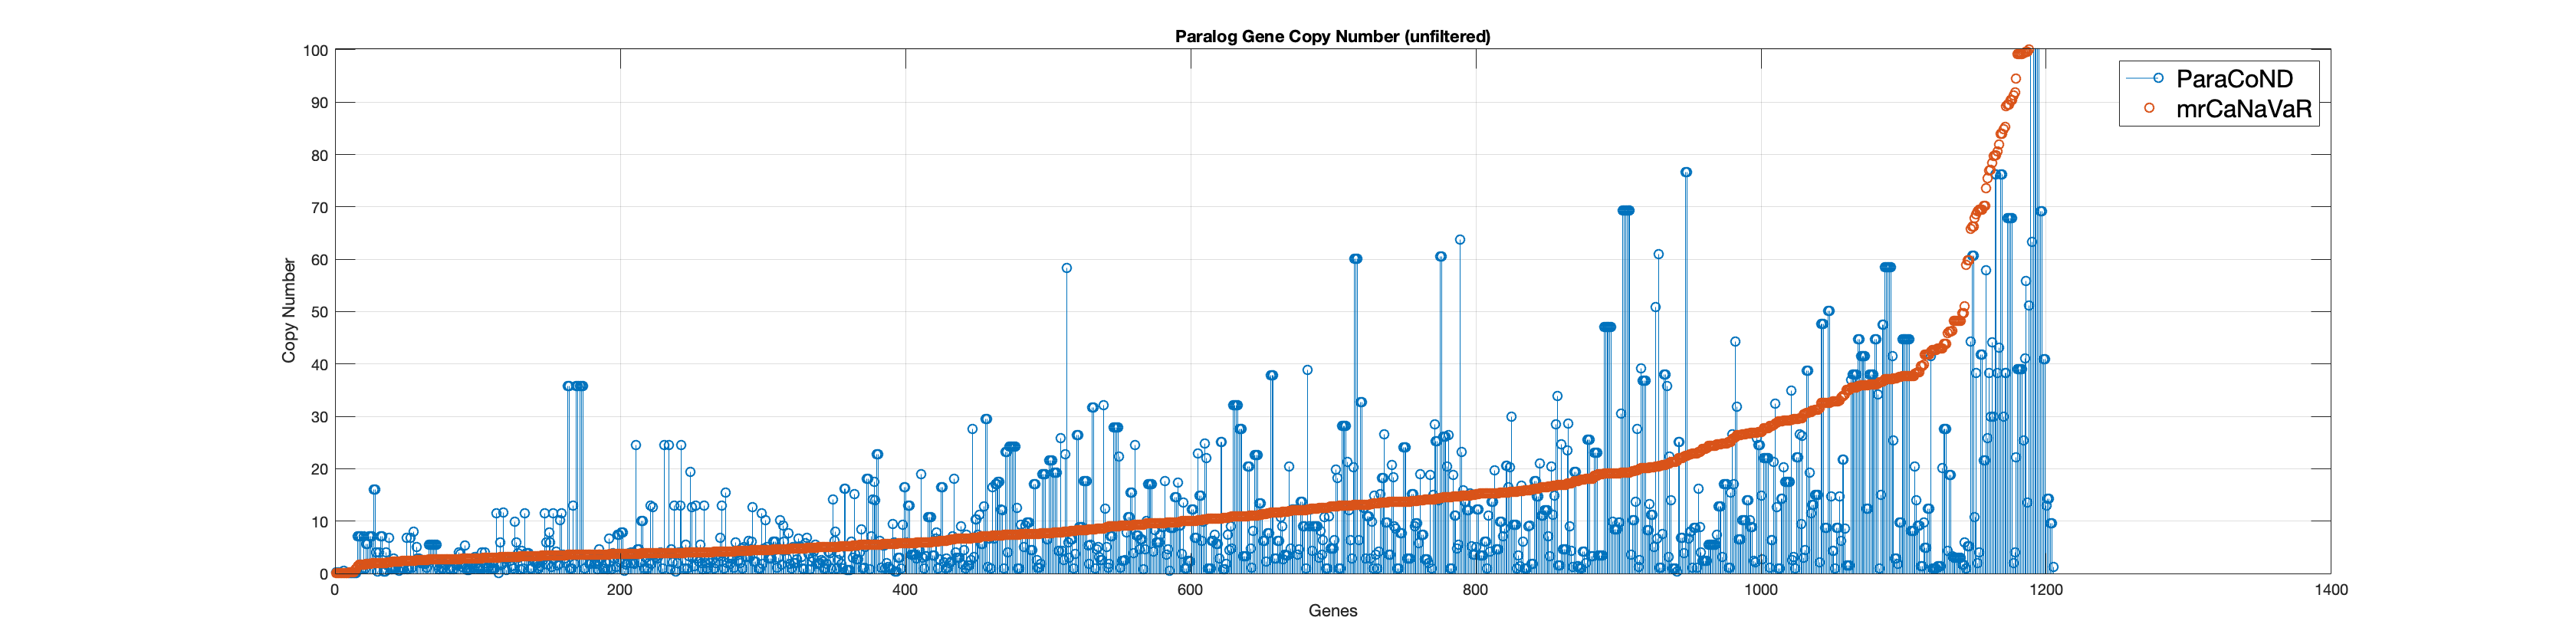
\includegraphics[scale=0.18]{images/na12878/figure1.png}\label{na12878unfiltered}}\quad
    \subfloat[42S291210]{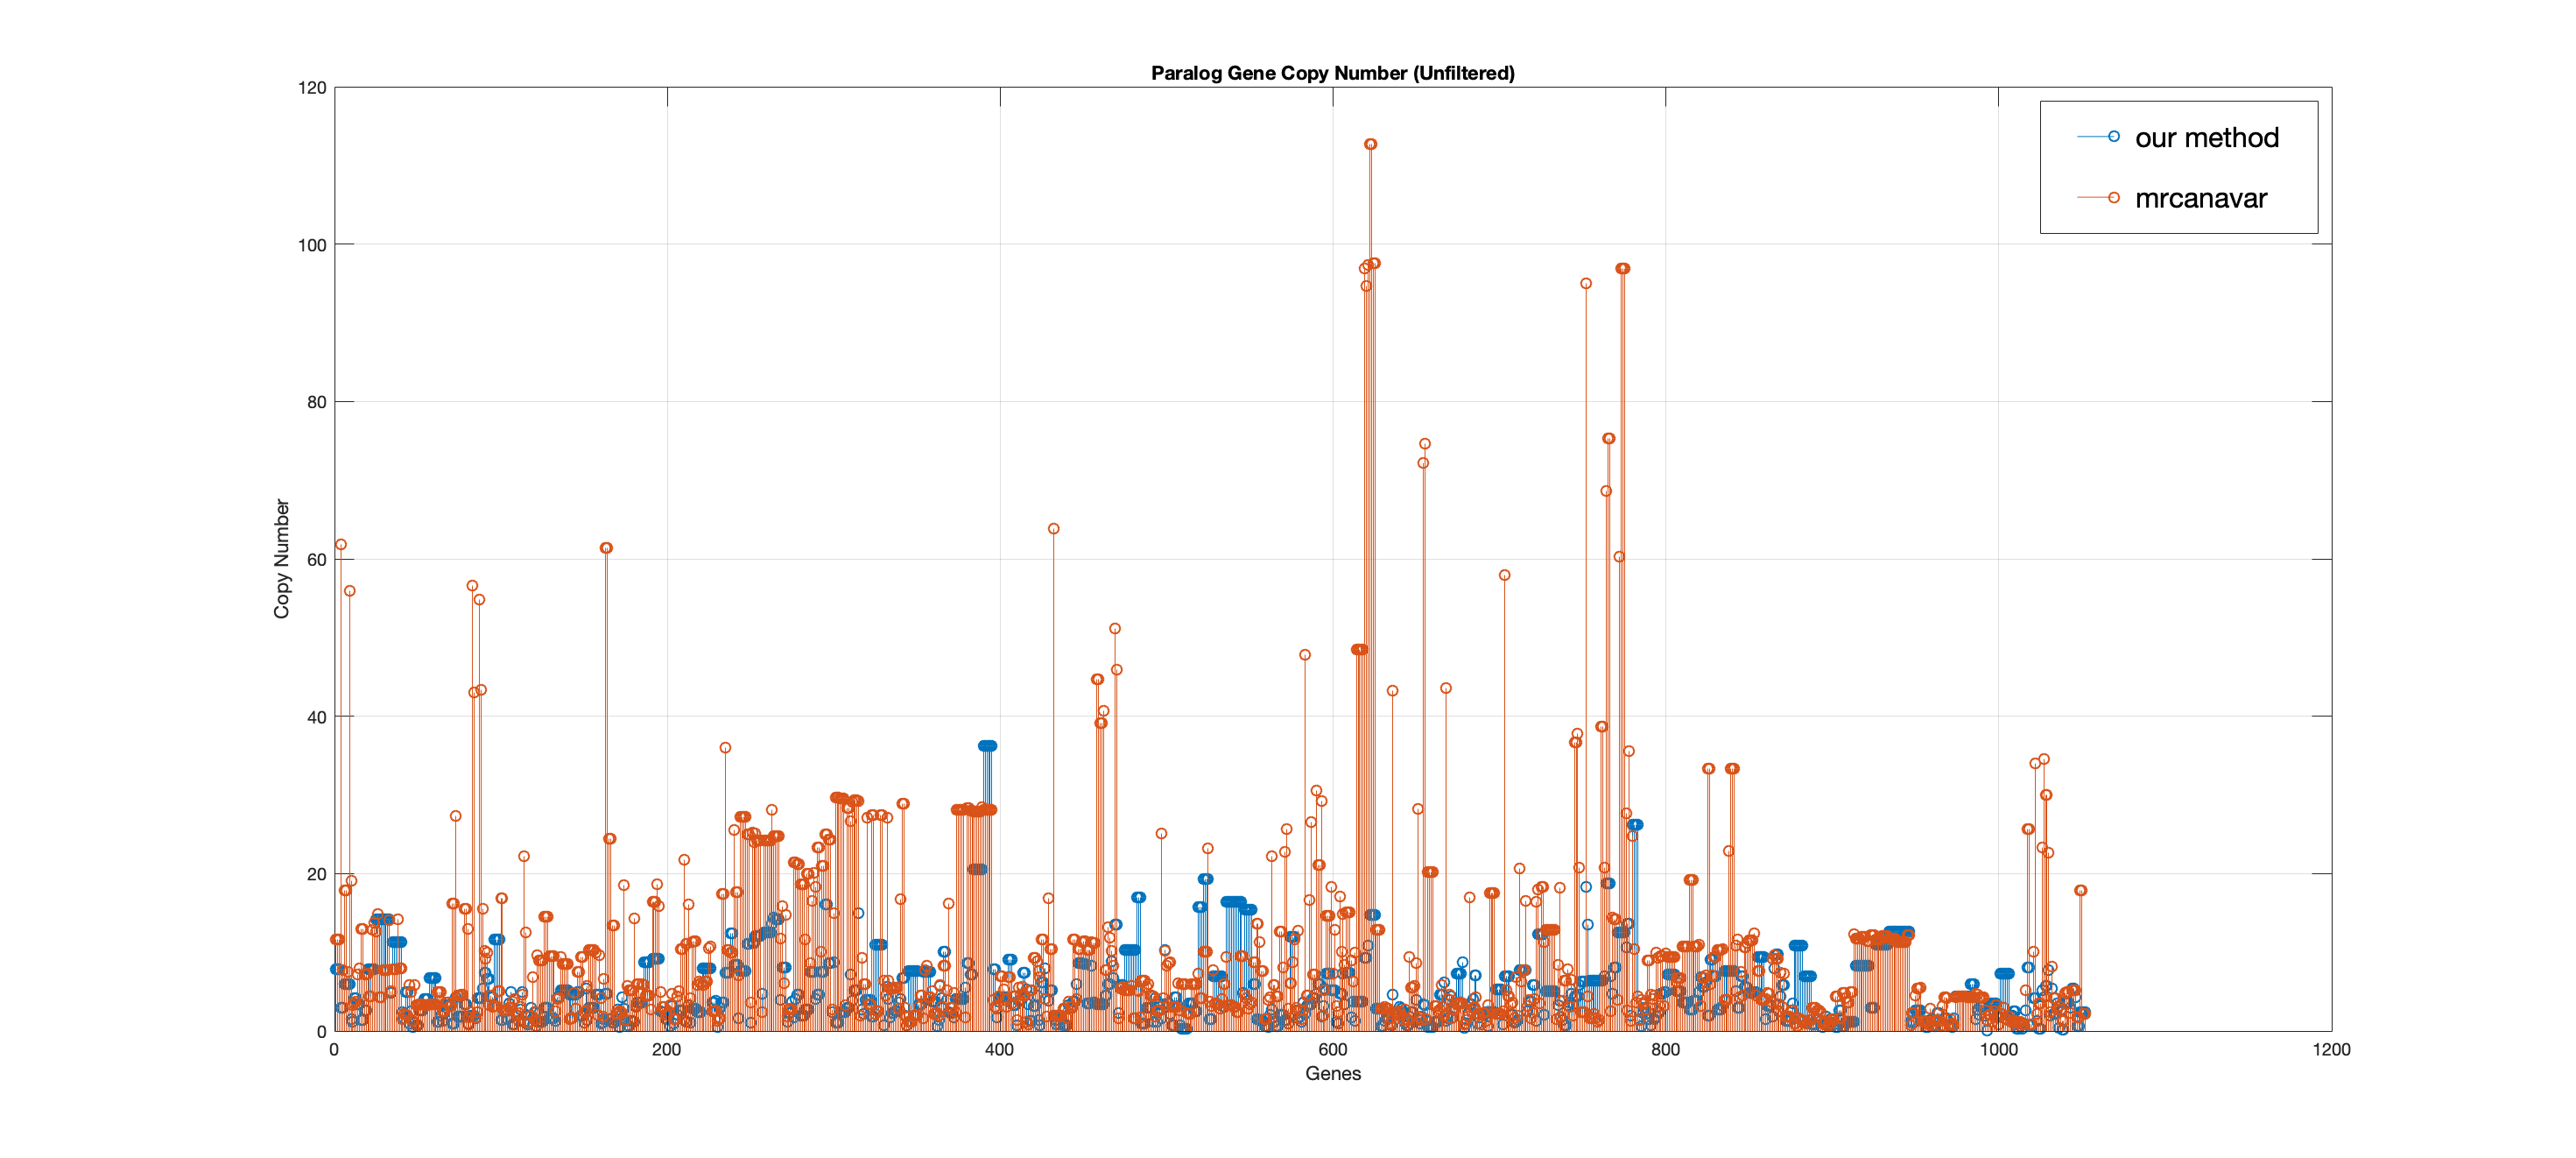
\includegraphics[scale=0.20]{images/42/figure1.png}\label{42unfiltered}}
    \caption{Absolute copy numbers of genes overlapping with segmental duplications}
    \label{unfiltered}
\end{sidewaysfigure}

\begin{figure}
    \centering
    \subfloat[NA12878]{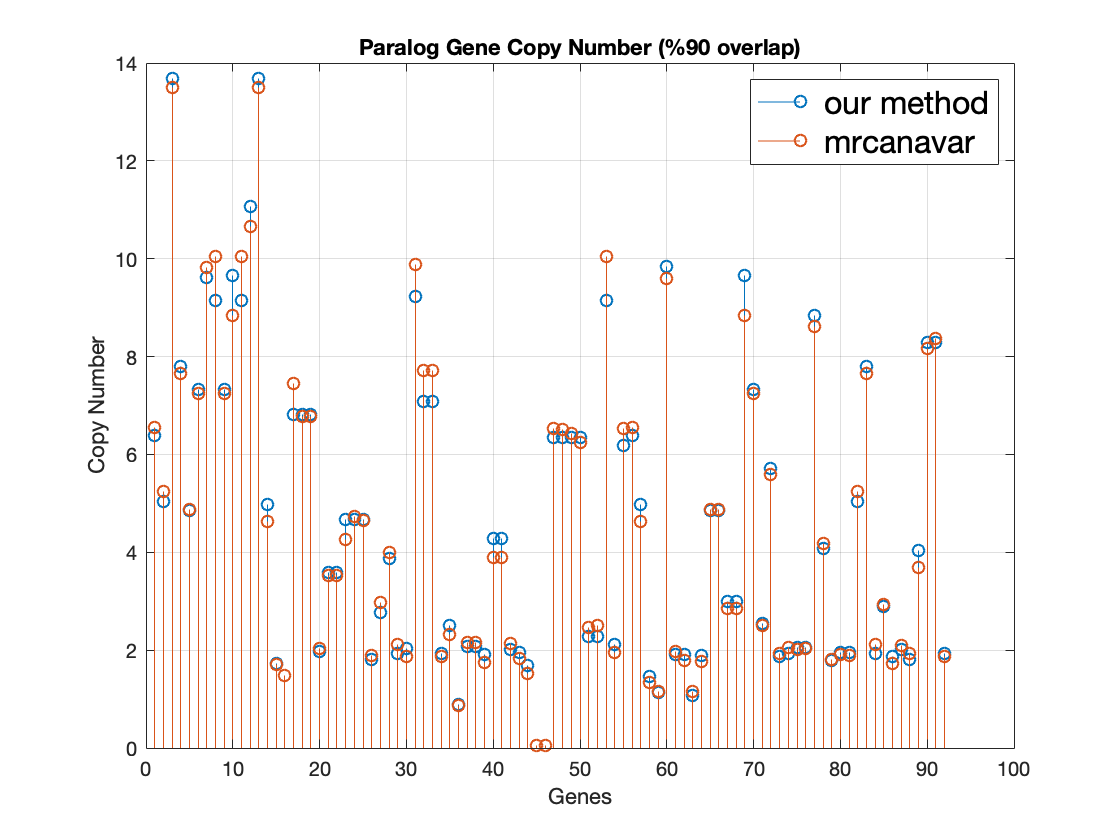
\includegraphics[scale=0.30]{images/na12878/figure2.png}\label{na12878overlap90}}\quad
    \subfloat[42S291210]{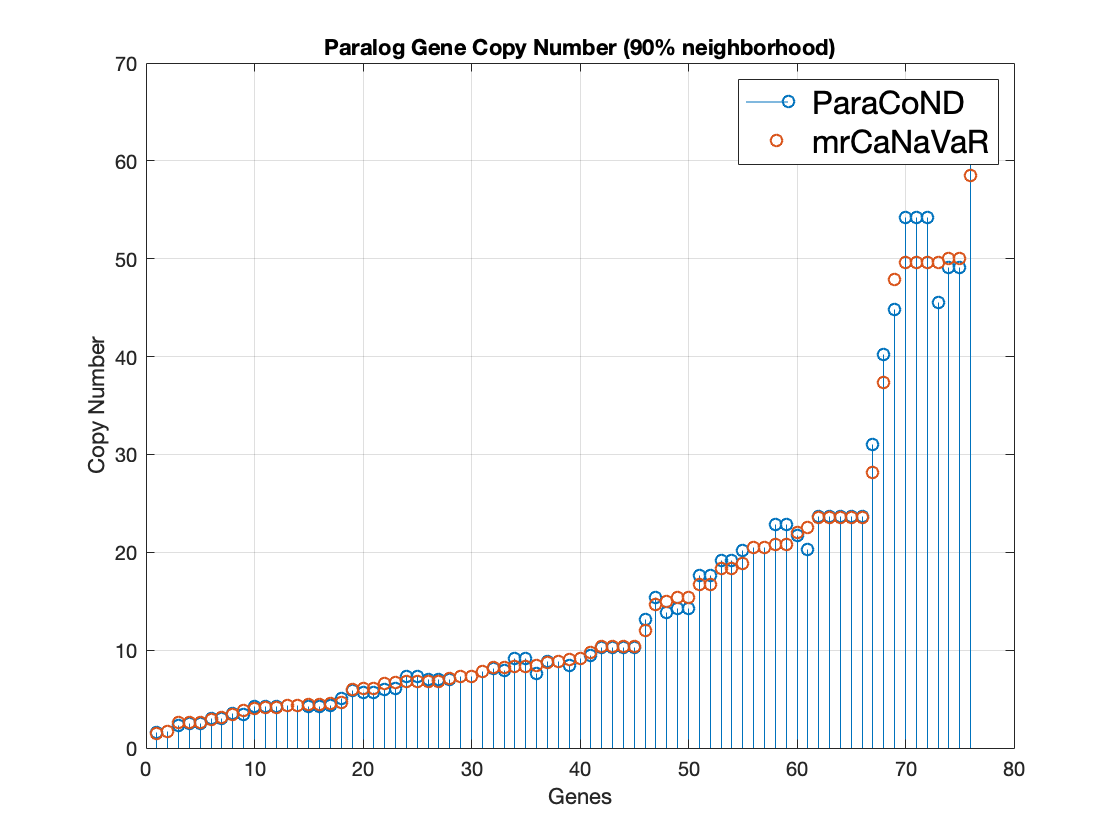
\includegraphics[scale=0.30]{images/42/figure2.png}\label{42overlap90}}
    \caption{Absolute copy numbers of genes showing \%90 overlapping by both methods}
    \label{overlap90}
\end{figure}

\begin{sidewaysfigure}[ht]
    \centering
    \subfloat[NA12878]{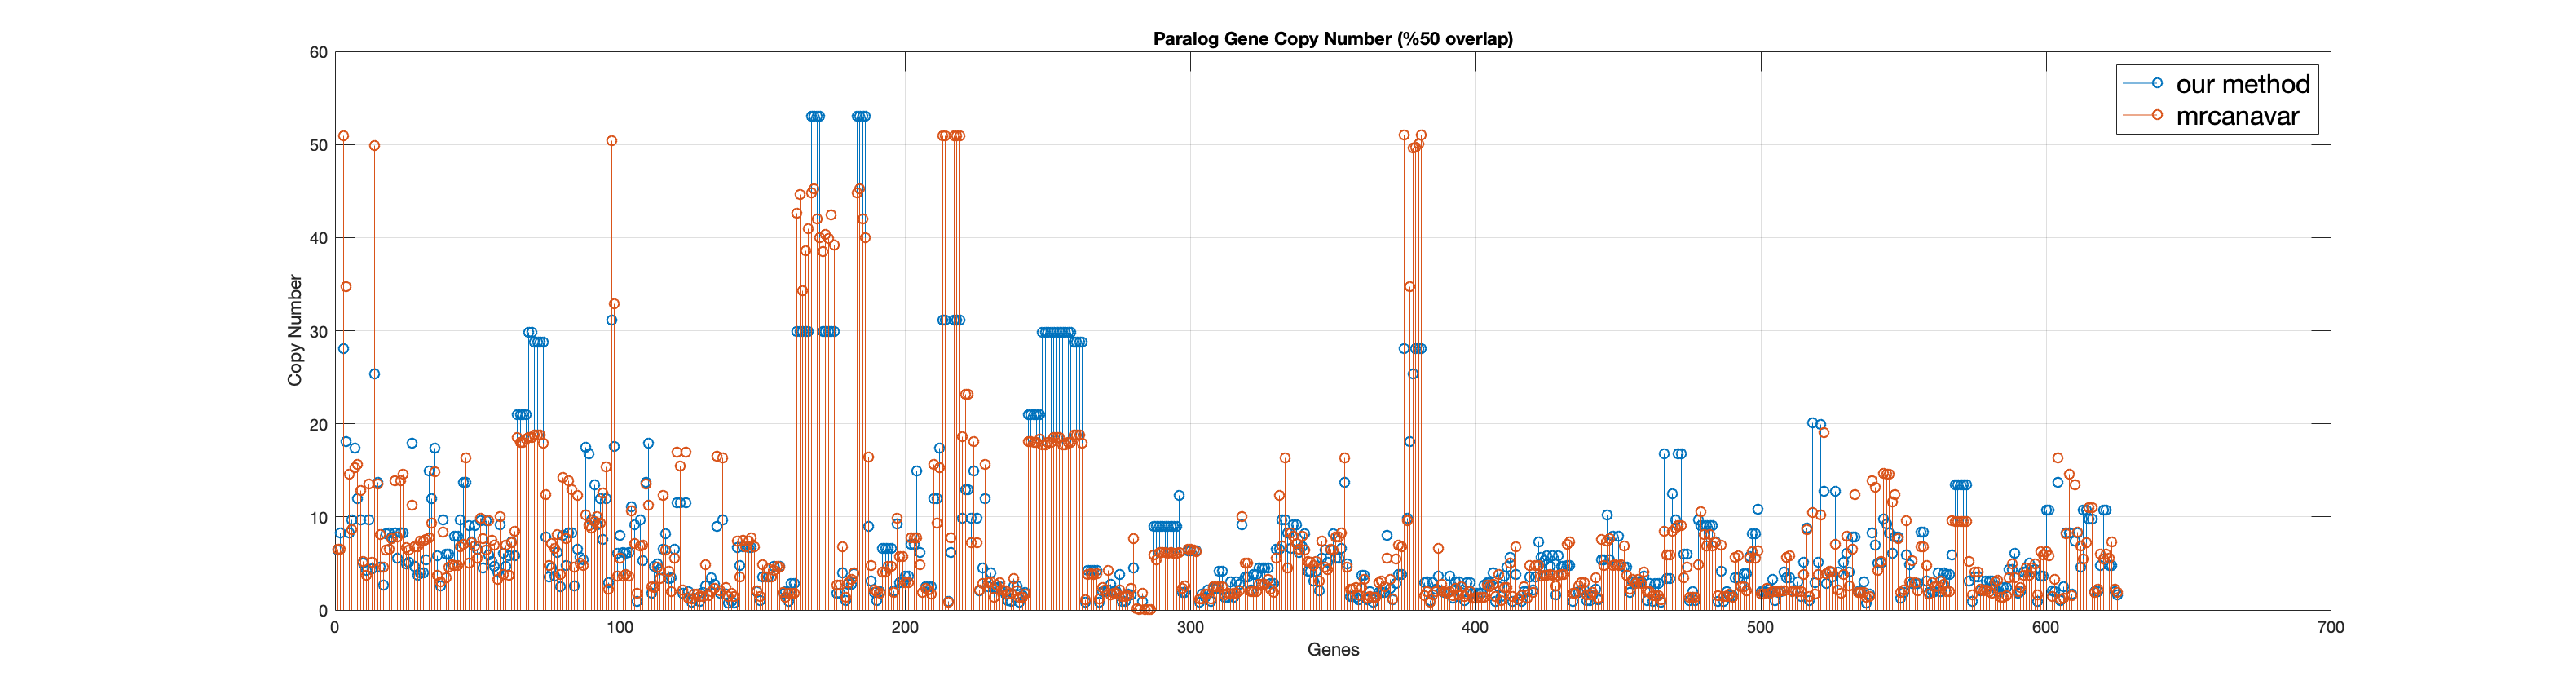
\includegraphics[scale=0.18]{images/na12878/figure3.png}\label{na12878overlap50}}\quad
    \subfloat[42S291210]{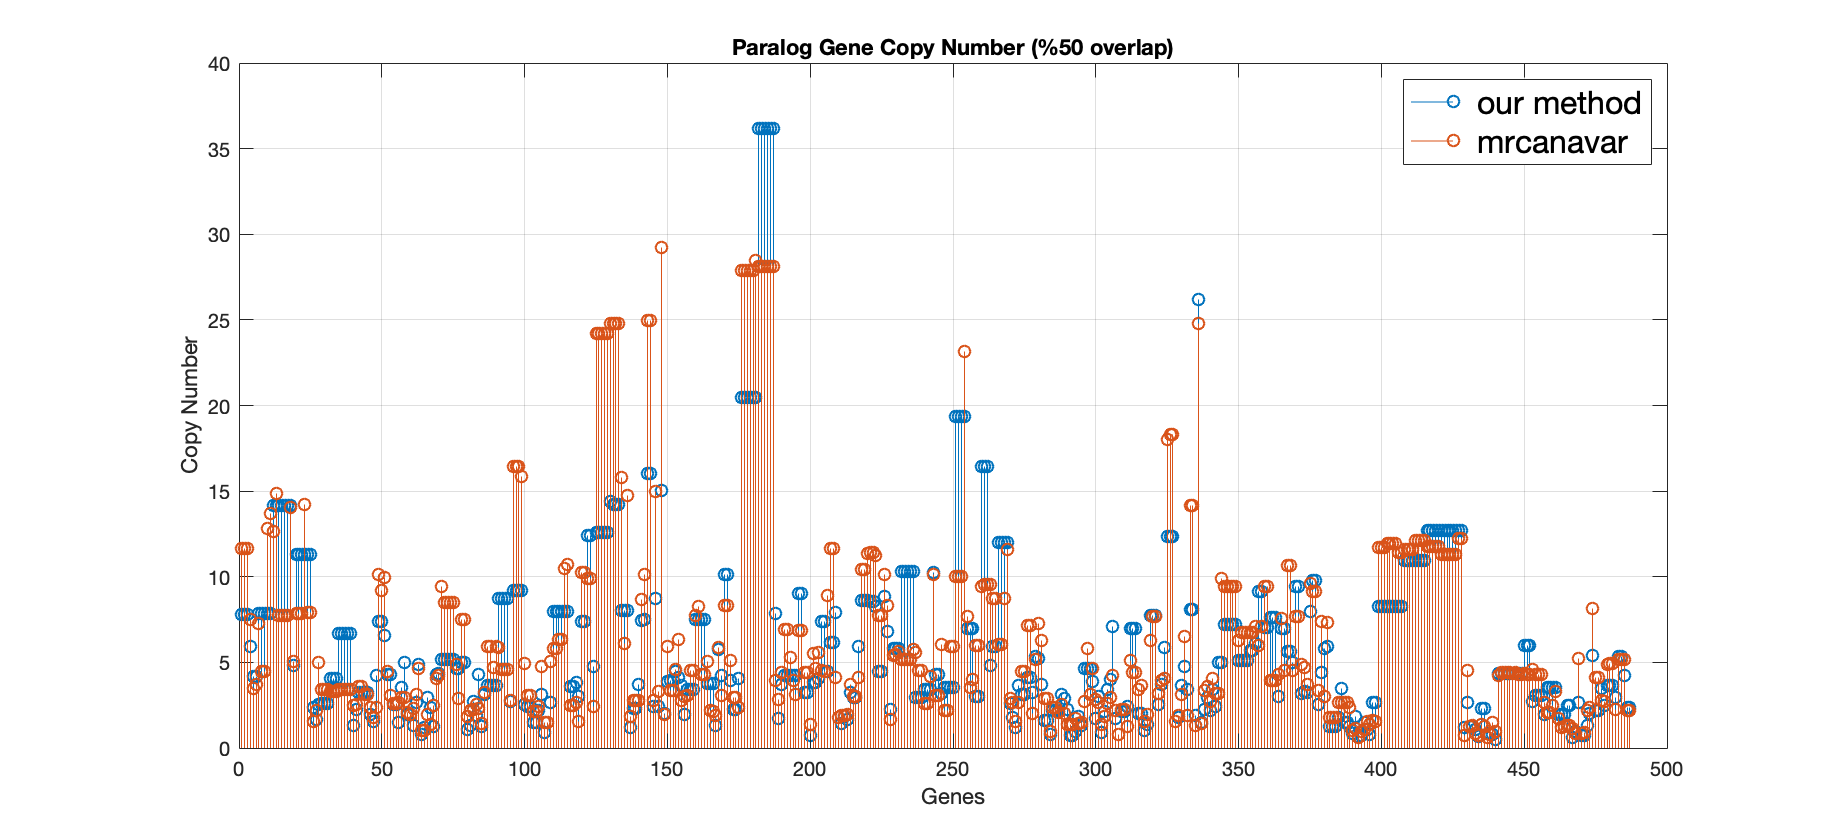
\includegraphics[scale=0.30]{images/42/figure3.png}\label{42overlap50}}
    \caption{Absolute copy numbers of genes showing \%50 overlapping by both methods}
    \label{overlap50}
\end{sidewaysfigure}


\begin{sidewaysfigure}[ht]
    \centering
    \subfloat[NA12878]{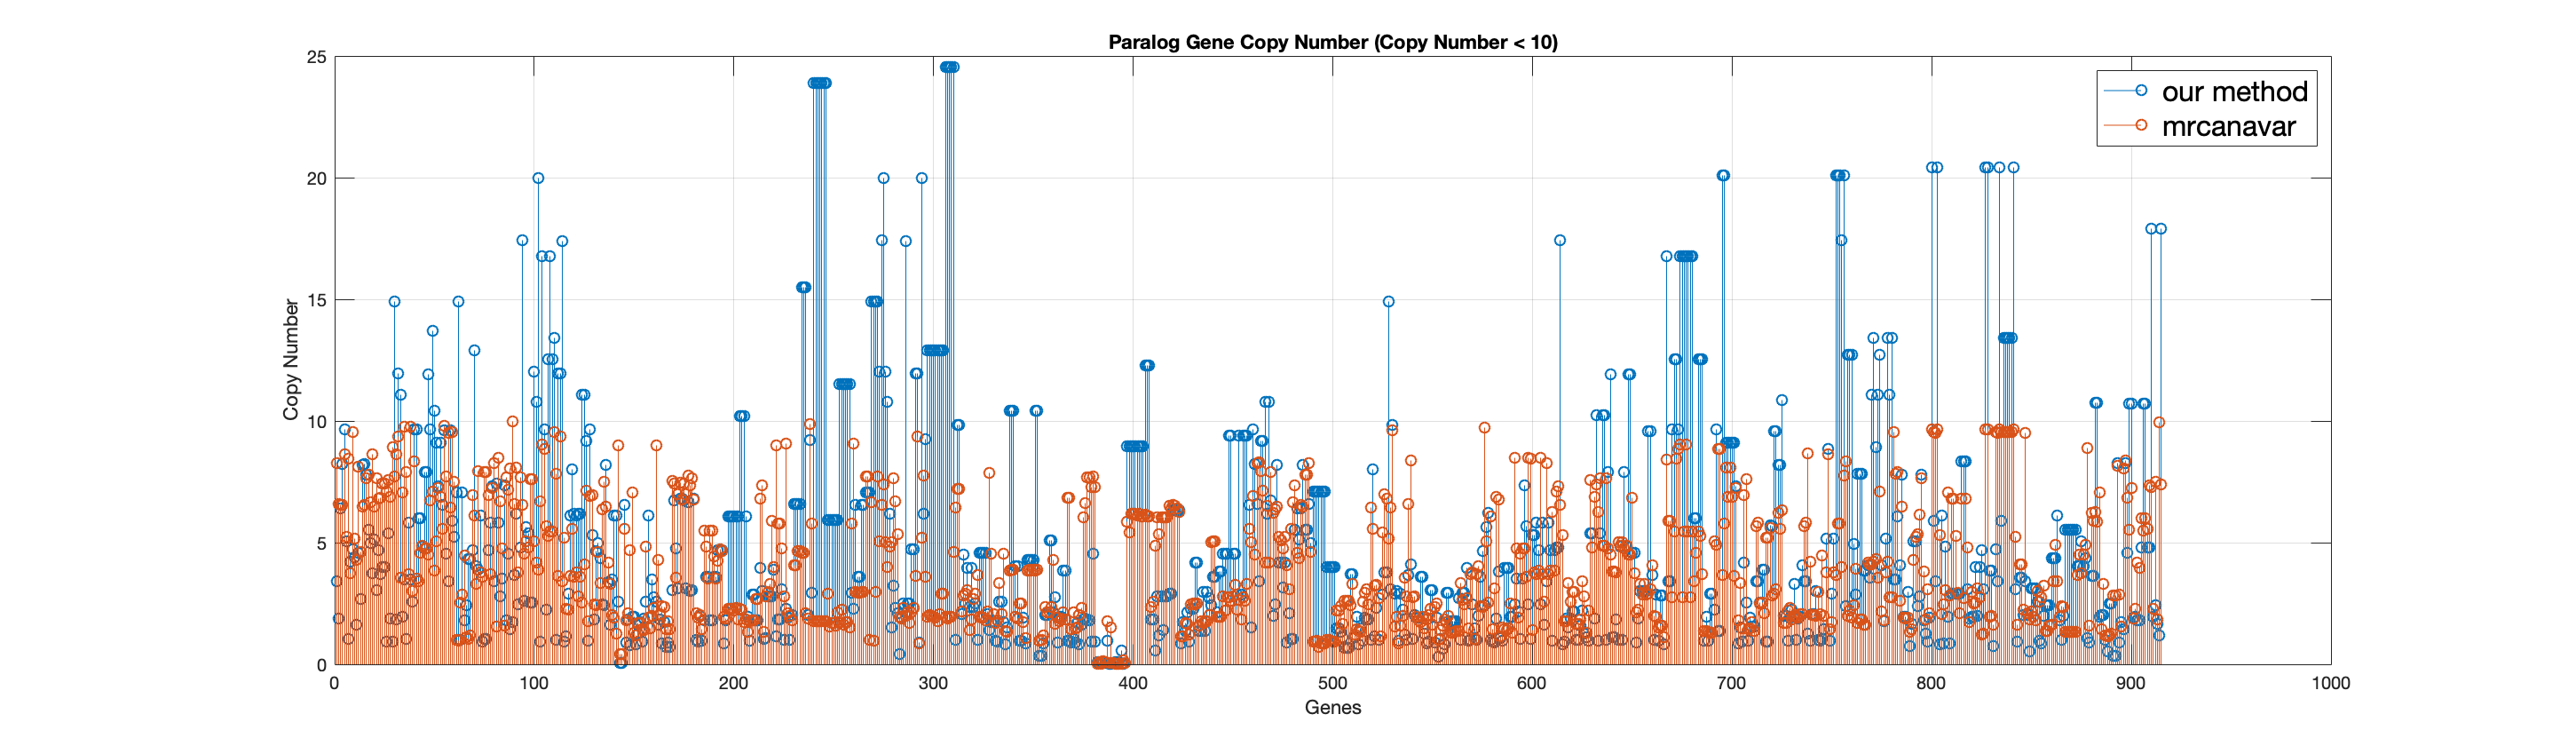
\includegraphics[scale=0.20]{images/na12878/figure4.png}\label{na12878lt10}}\quad
    \subfloat[42S291210]{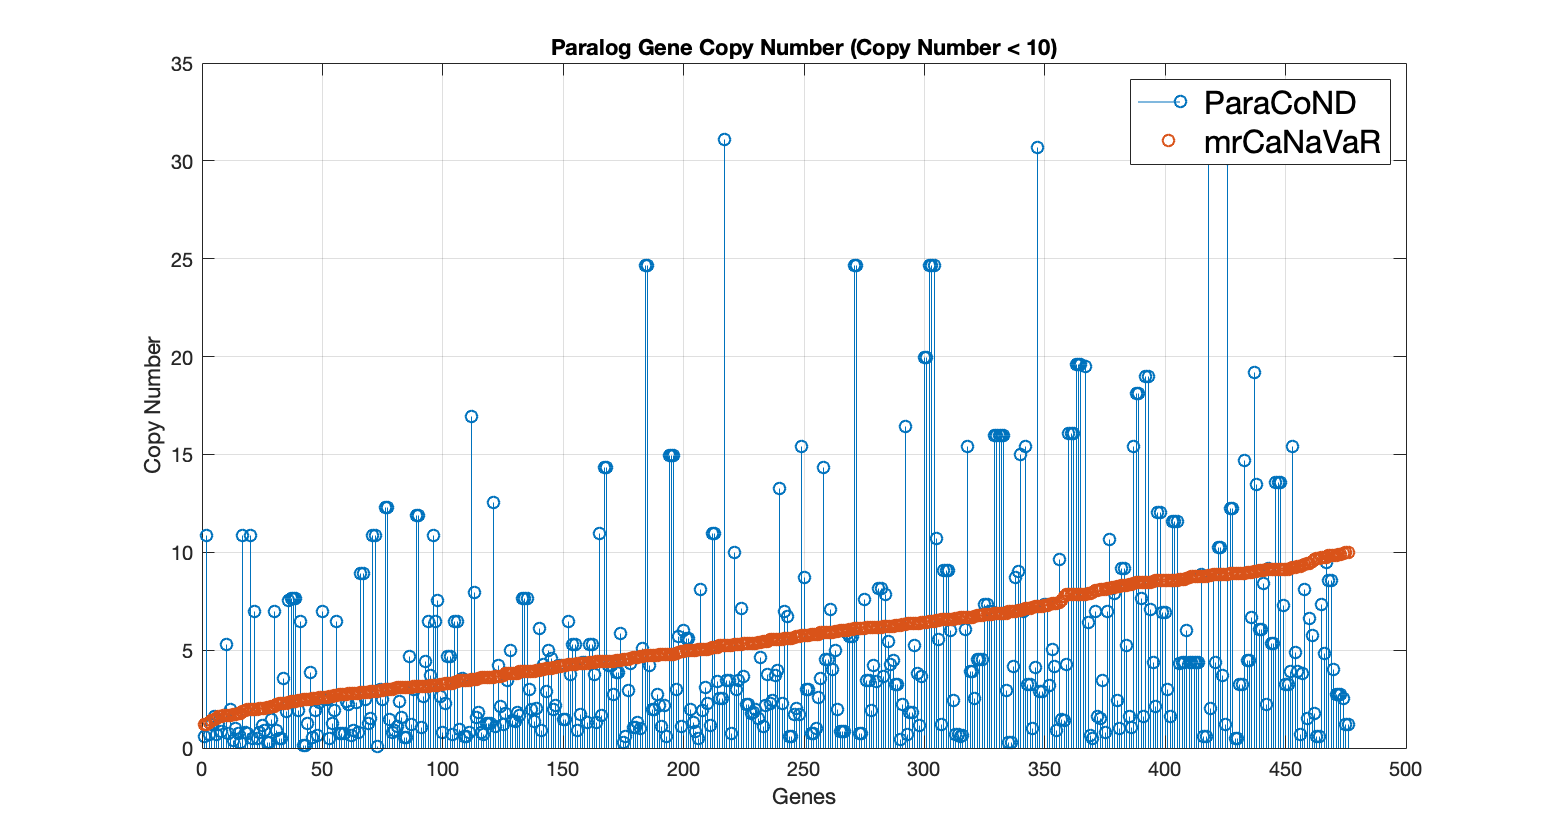
\includegraphics[scale=0.20]{images/42/figure4.png}\label{42lt10}}
    \caption{Absolute copy numbers of genes whose copy numbers are less than 10 according to mrCaNaVaR}
    \label{lessThan10}
\end{sidewaysfigure}

\begin{figure}
    \centering
    \subfloat[NA12878]{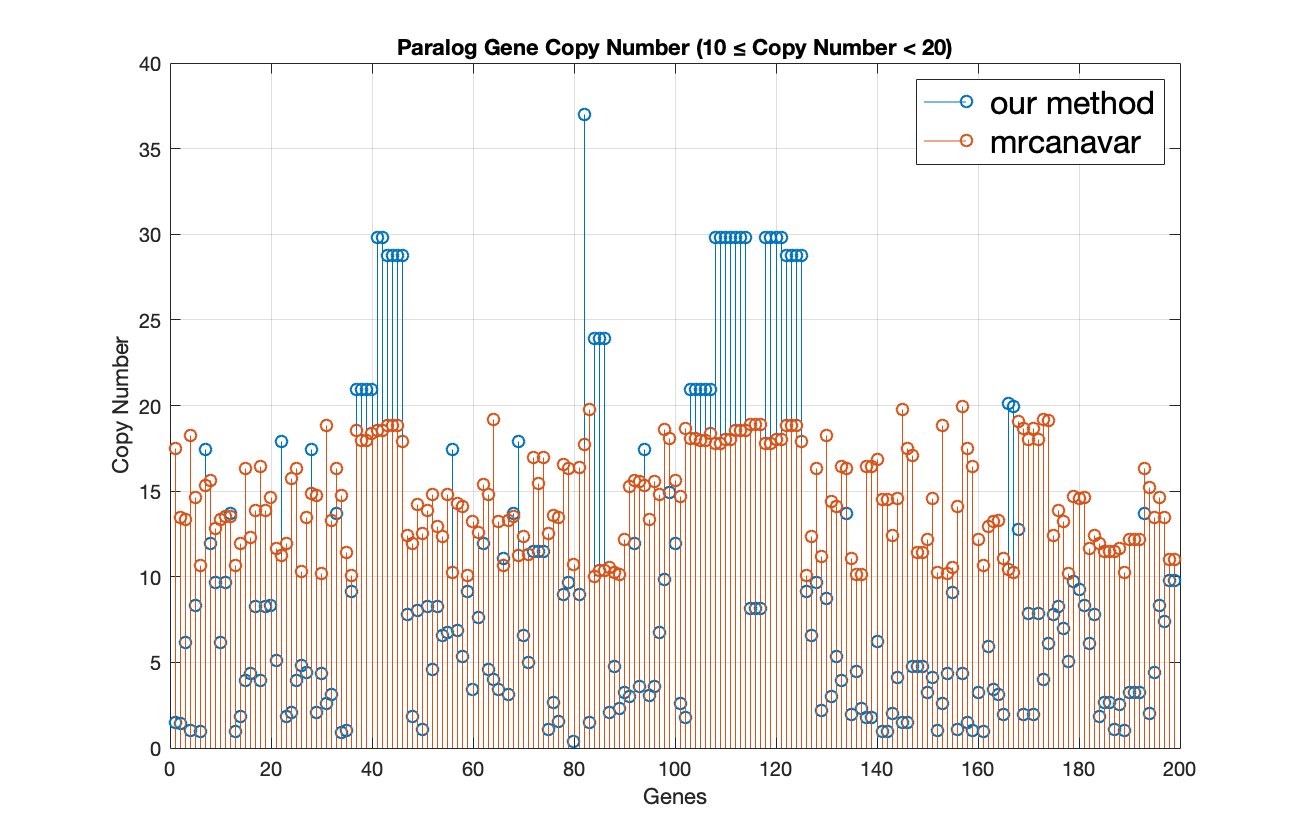
\includegraphics[scale=0.30]{images/na12878/figure5.png}\label{na12878btw1020}}\quad
    \subfloat[42S291210]{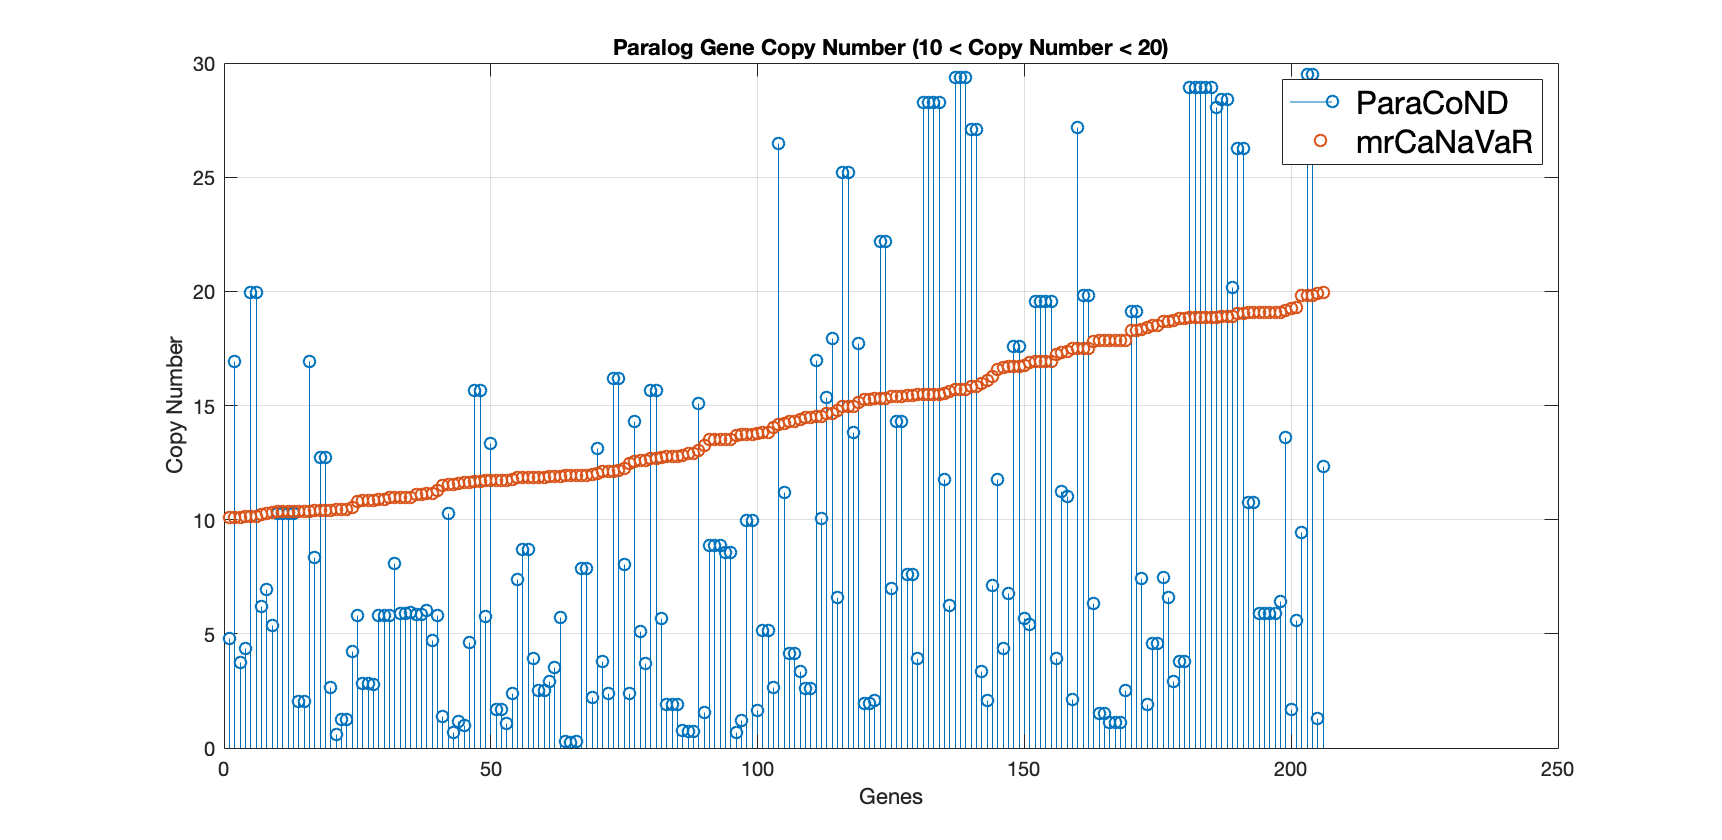
\includegraphics[scale=0.25]{images/42/figure5.png}\label{42btw1020}}
    \caption{Absolute copy numbers of genes whose copy numbers are between 10 and 20 according to mrCaNaVaR}
    \label{btw2030}
\end{figure}


\begin{figure}
    \centering
    \subfloat[NA12878]{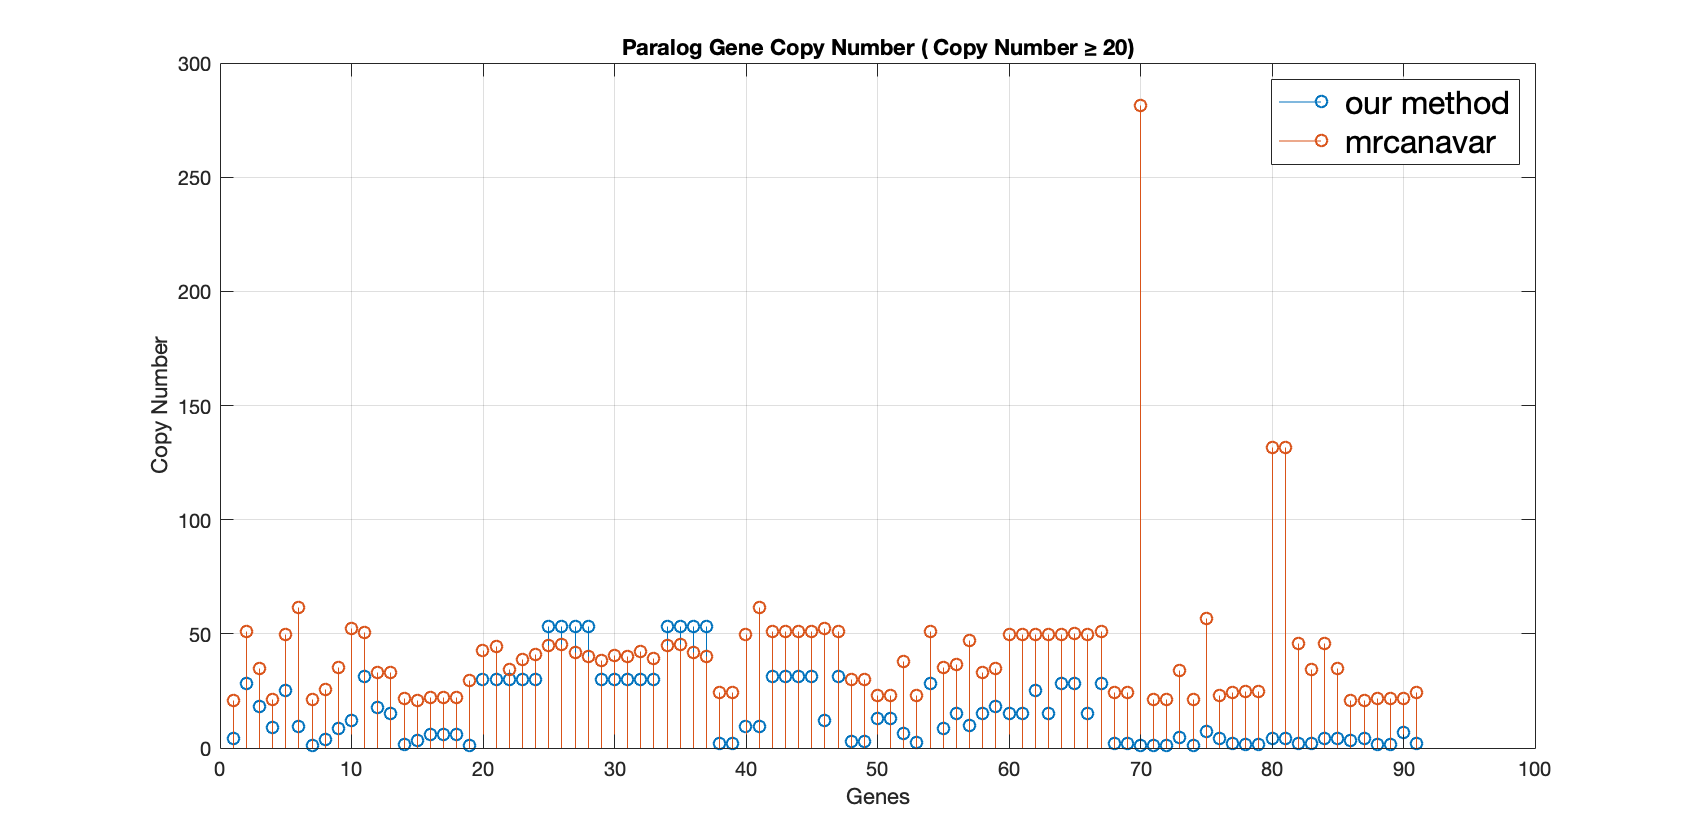
\includegraphics[scale=0.25]{images/na12878/figure6.png}\label{na12878gt20}}\quad
    \subfloat[42S291210]{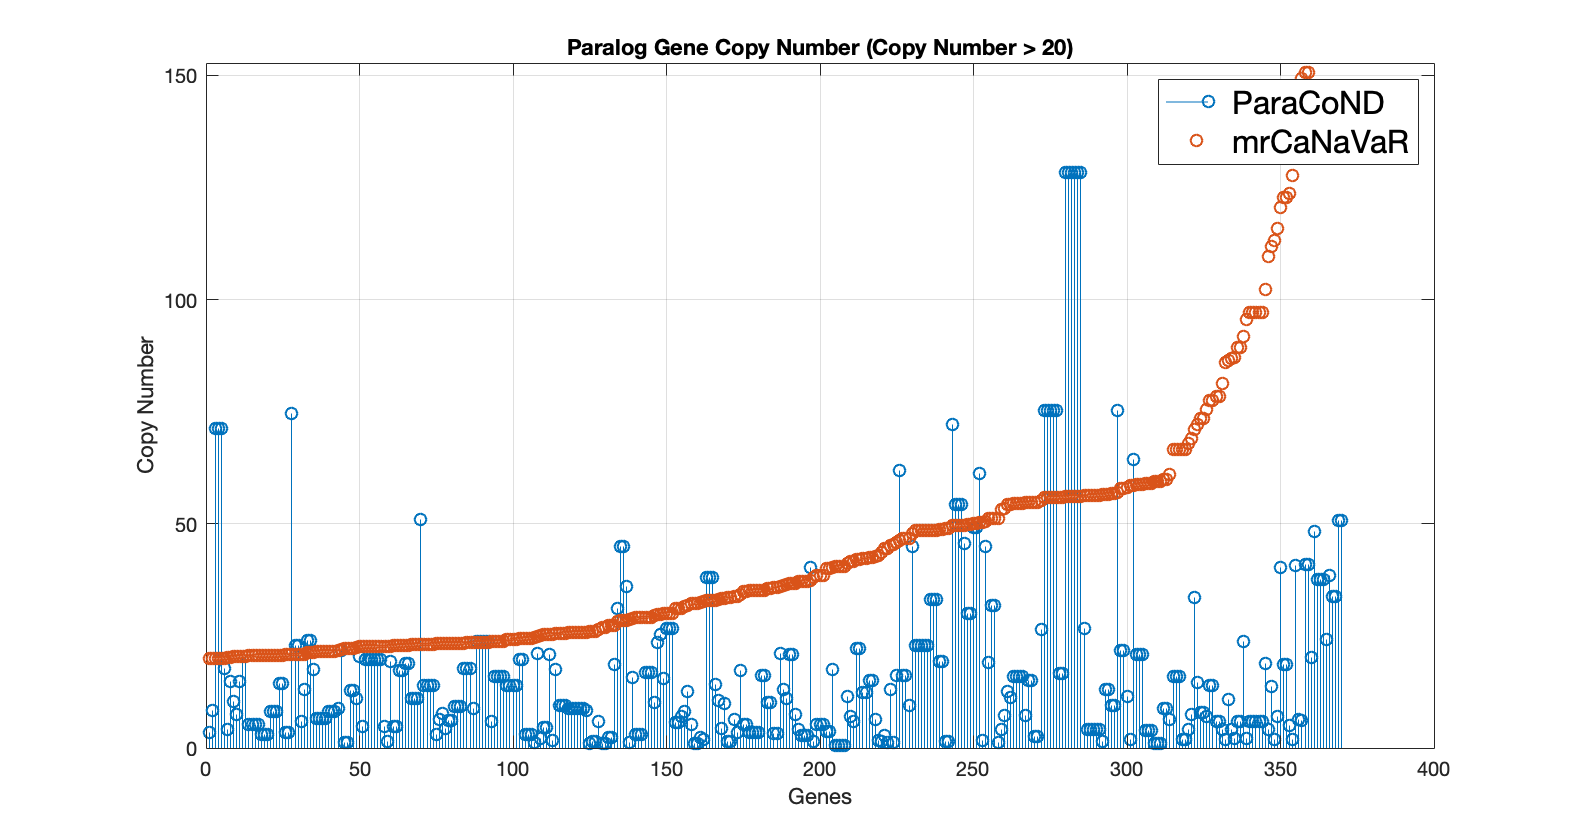
\includegraphics[scale=0.20]{images/42/figure6.png}\label{42gt20}}
    \caption{Absolute copy numbers of genes whose copy numbers are greater than 20 according to mrCaNaVaR}
    \label{greaterThan20}
\end{figure}